\setcounter{definition}{0} \setcounter{property}{0} \setcounter{claim}{0} \setcounter{fact}{0} \setcounter{corollary}{0} \setcounter{figure}{0}
\section{Minimum Spanning Tree}

\subsection*{Tree and Spanning Tree}

A tree is an undirected graph that is connected and acyclic.
(``connected'' here means the graph consists of a single connected component.)
A tree $T = (V, E)$ always satisfies that $|E| = |V| - 1$.
In fact, any two of these three properties~(i.e., connected, acyclic, and $|E| = |V| - 1$)
implies the other one, formally stated below. Play with some examples
to fully understand these properties.

\begin{fact}\label{mst-fact1}
Let $T = (V, E)$ be an undirected graph. The following statements are equivalent.
\vspace*{-\topsep}
\begin{enumerate}
\item $T$ is a tree.
\item $T$ is connected and acyclic.
\item $|E| = |V| - 1$ and $T$ is acyclic.
\item $|E| = |V| - 1$ and $T$ is connected.
\item There exists an unique path between every pair of vertices of $T$.
\end{enumerate}
\end{fact}

Let $G = (V,E)$ be an undirected graph.
We say tree $T = (V_1, E_1)$ is a \emph{spanning tree}
of $G$ if $V_1 = V$ and $E_1\subset E$.
As $T$ is a tree, clearly we have $|E_1| = |V_1| - 1 = |V| - 1$.
Note that a spanning tree is always w.r.t.\ a graph, i.e., we always
say a spanning tree of a graph. Note too, that for an undirected graph $G$, 
its spanning tree may not be unqiue. See Figure~\ref{fig:mst-spanning}
for an example.  (Think: when an undirected graph has a unique spanning tree?)

\begin{figure}[h]
\centering{

\tikzset{every picture/.style={line width=0.75pt}} %set default line width to 0.75pt        

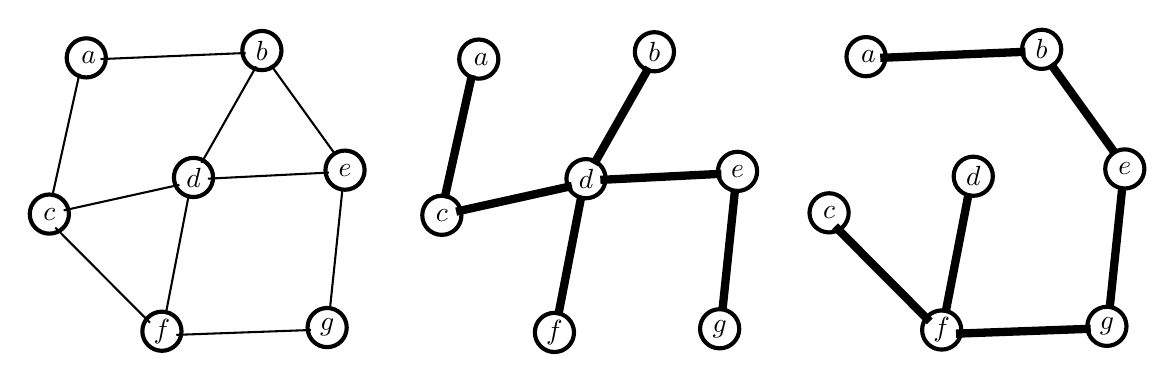
\begin{tikzpicture}[x=0.5pt,y=0.5pt,yscale=-1,xscale=1]
%uncomment if require: \path (0,290); %set diagram left start at 0, and has height of 290

%Straight Lines [id:da6859712806144006] 
\draw [color={rgb, 255:red, 0; green, 0; blue, 0 }  ,draw opacity=1 ][line width=0.75]    (185,39.17) -- (231.39,103.54) ;
%Straight Lines [id:da43828905709564314] 
\draw [color={rgb, 255:red, 0; green, 0; blue, 0 }  ,draw opacity=1 ][line width=0.75]    (116.55,234.06) -- (213.9,230.54) ;
%Straight Lines [id:da6385368954330931] 
\draw [color={rgb, 255:red, 0; green, 0; blue, 0 }  ,draw opacity=1 ][line width=0.75]    (29.1,156.46) -- (97.54,225.24) ;
%Straight Lines [id:da061278223687582845] 
\draw [color={rgb, 255:red, 0; green, 0; blue, 0 }  ,draw opacity=1 ][line width=0.75]    (35.18,144.11) -- (118.84,125.59) ;
%Straight Lines [id:da125058897644165] 
\draw [color={rgb, 255:red, 0; green, 0; blue, 0 }  ,draw opacity=1 ][line width=0.75]    (46.59,45.34) -- (26.81,134.41) ;
%Straight Lines [id:da7561477389708726] 
\draw [color={rgb, 255:red, 0; green, 0; blue, 0 }  ,draw opacity=1 ][line width=0.75]    (61.8,34.76) -- (166.75,30.35) ;
%Straight Lines [id:da8045438090716241] 
\draw [color={rgb, 255:red, 0; green, 0; blue, 0 }  ,draw opacity=1 ][line width=0.75]    (174.35,40.05) -- (134.81,109.72) ;
%Straight Lines [id:da7384444755679203] 
\draw [color={rgb, 255:red, 0; green, 0; blue, 0 }  ,draw opacity=1 ][line width=0.75]    (125.68,132.65) -- (108.95,219.07) ;
%Straight Lines [id:da7781378597799559] 
\draw [color={rgb, 255:red, 0; green, 0; blue, 0 }  ,draw opacity=1 ][line width=0.75]    (236.71,128.24) -- (227.59,215.54) ;
%Straight Lines [id:da6283012441188964] 
\draw [color={rgb, 255:red, 0; green, 0; blue, 0 }  ,draw opacity=1 ][line width=0.75]    (226.83,116.77) -- (139.37,121.18) ;
%Straight Lines [id:da438892015392218] 
\draw [color={rgb, 255:red, 0; green, 0; blue, 0 }  ,draw opacity=1 ][line width=3]    (318.85,144.99) -- (402.51,126.47) ;
%Straight Lines [id:da8359945945218459] 
\draw [color={rgb, 255:red, 0; green, 0; blue, 0 }  ,draw opacity=1 ][line width=3]    (330.26,46.22) -- (310.48,135.29) ;
%Straight Lines [id:da21420370300632352] 
\draw [color={rgb, 255:red, 0; green, 0; blue, 0 }  ,draw opacity=1 ][line width=3]    (458.02,40.93) -- (418.48,110.6) ;
%Straight Lines [id:da9239671202801586] 
\draw [color={rgb, 255:red, 0; green, 0; blue, 0 }  ,draw opacity=1 ][line width=3]    (409.35,133.53) -- (392.62,219.95) ;
%Straight Lines [id:da821215549767216] 
\draw [color={rgb, 255:red, 0; green, 0; blue, 0 }  ,draw opacity=1 ][line width=3]    (520.38,129.12) -- (511.26,216.43) ;
%Straight Lines [id:da9218980242104106] 
\draw [color={rgb, 255:red, 0; green, 0; blue, 0 }  ,draw opacity=1 ][line width=3]    (510.5,117.65) -- (423.04,122.06) ;
%Straight Lines [id:da35247521934474646] 
\draw [color={rgb, 255:red, 0; green, 0; blue, 0 }  ,draw opacity=1 ][line width=3]    (748.54,38.28) -- (794.93,102.66) ;
%Straight Lines [id:da7944029026500893] 
\draw [color={rgb, 255:red, 0; green, 0; blue, 0 }  ,draw opacity=1 ][line width=3]    (680.09,233.18) -- (777.44,229.65) ;
%Straight Lines [id:da39283588857656926] 
\draw [color={rgb, 255:red, 0; green, 0; blue, 0 }  ,draw opacity=1 ][line width=3]    (592.63,155.57) -- (661.08,224.36) ;
%Straight Lines [id:da24731320696047454] 
\draw [color={rgb, 255:red, 0; green, 0; blue, 0 }  ,draw opacity=1 ][line width=3]    (625.33,33.87) -- (730.28,29.46) ;
%Straight Lines [id:da24545478407911292] 
\draw [color={rgb, 255:red, 0; green, 0; blue, 0 }  ,draw opacity=1 ][line width=3]    (689.22,131.76) -- (672.49,218.19) ;
%Straight Lines [id:da379919078999982] 
\draw [color={rgb, 255:red, 0; green, 0; blue, 0 }  ,draw opacity=1 ][line width=3]    (800.25,127.35) -- (791.12,214.66) ;

% Text Node
\draw  [line width=1.5]   (238.52, 115.01) circle [x radius= 14.15, y radius= 14.15]   ;
\draw (238.52,115.01) node   [align=left] {$\displaystyle e$};
% Text Node
\draw  [line width=1.5]   (51.52, 33.87) circle [x radius= 14.15, y radius= 14.15]   ;
\draw (46.02,33.87) node [anchor=west] [inner sep=0.75pt]   [align=left] {$\displaystyle a$};
% Text Node
\draw  [line width=1.5]   (178.44, 28.58) circle [x radius= 14.15, y radius= 14.15]   ;
\draw (178.44,28.58) node   [align=left] {$\displaystyle b$};
% Text Node
\draw  [line width=1.5]   (24.82, 146.76) circle [x radius= 14.15, y radius= 14.15]   ;
\draw (24.82,146.76) node   [align=left] {$\displaystyle c$};
% Text Node
\draw  [line width=1.5]   (129.01, 120.3) circle [x radius= 14.15, y radius= 14.15]   ;
\draw (129.01,120.3) node   [align=left] {$\displaystyle d$};
% Text Node
\draw  [line width=1.5]   (106.19, 231.42) circle [x radius= 14.15, y radius= 14.15]   ;
\draw (106.19,231.42) node   [align=left] {$\displaystyle f$};
% Text Node
\draw  [line width=1.5]   (225.59, 228.77) circle [x radius= 14.15, y radius= 14.15]   ;
\draw (225.59,228.77) node   [align=left] {$\displaystyle g$};
% Text Node
\draw  [line width=1.5]   (522.19, 115.89) circle [x radius= 14.15, y radius= 14.15]   ;
\draw (522.19,115.89) node   [align=left] {$\displaystyle e$};
% Text Node
\draw  [line width=1.5]   (335.19, 34.76) circle [x radius= 14.15, y radius= 14.15]   ;
\draw (329.69,34.76) node [anchor=west] [inner sep=0.75pt]   [align=left] {$\displaystyle a$};
% Text Node
\draw  [line width=1.5]   (462.11, 29.46) circle [x radius= 14.15, y radius= 14.15]   ;
\draw (462.11,29.46) node   [align=left] {$\displaystyle b$};
% Text Node
\draw  [line width=1.5]   (308.49, 147.64) circle [x radius= 14.15, y radius= 14.15]   ;
\draw (308.49,147.64) node   [align=left] {$\displaystyle c$};
% Text Node
\draw  [line width=1.5]   (412.68, 121.18) circle [x radius= 14.15, y radius= 14.15]   ;
\draw (412.68,121.18) node   [align=left] {$\displaystyle d$};
% Text Node
\draw  [line width=1.5]   (389.86, 232.3) circle [x radius= 14.15, y radius= 14.15]   ;
\draw (389.86,232.3) node   [align=left] {$\displaystyle f$};
% Text Node
\draw  [line width=1.5]   (509.26, 229.65) circle [x radius= 14.15, y radius= 14.15]   ;
\draw (509.26,229.65) node   [align=left] {$\displaystyle g$};
% Text Node
\draw  [line width=1.5]   (802.06, 114.13) circle [x radius= 14.15, y radius= 14.15]   ;
\draw (802.06,114.13) node   [align=left] {$\displaystyle e$};
% Text Node
\draw  [line width=1.5]   (615.06, 32.99) circle [x radius= 14.15, y radius= 14.15]   ;
\draw (609.56,32.99) node [anchor=west] [inner sep=0.75pt]   [align=left] {$\displaystyle a$};
% Text Node
\draw  [line width=1.5]   (741.98, 27.7) circle [x radius= 14.15, y radius= 14.15]   ;
\draw (741.98,27.7) node   [align=left] {$\displaystyle b$};
% Text Node
\draw  [line width=1.5]   (588.35, 145.87) circle [x radius= 14.15, y radius= 14.15]   ;
\draw (588.35,145.87) node   [align=left] {$\displaystyle c$};
% Text Node
\draw  [line width=1.5]   (692.54, 119.42) circle [x radius= 14.15, y radius= 14.15]   ;
\draw (692.54,119.42) node   [align=left] {$\displaystyle d$};
% Text Node
\draw  [line width=1.5]   (669.73, 230.54) circle [x radius= 14.15, y radius= 14.15]   ;
\draw (669.73,230.54) node   [align=left] {$\displaystyle f$};
% Text Node
\draw  [line width=1.5]   (789.13, 227.89) circle [x radius= 14.15, y radius= 14.15]   ;
\draw (789.13,227.89) node   [align=left] {$\displaystyle g$};


\end{tikzpicture}

}
\caption{Two spanning trees~(middle and right) of an undirected graph~(left).}
\label{fig:mst-spanning}
\end{figure}

By above definition, a spanning tree of $G = (V,E)$ is a tree that uses $(|V| - 1)$ edges
of $G$ that connects all vertices of $G$.
Following Fact~\ref{mst-fact1}, we can construct a spanning tree of $G$
in the following two ways:
\vspace*{-\topsep}
\begin{enumerate}
\item pick $(|V|-1)$ edges of $G$ that are acyclic;
\item pick $(|V|-1)$ edges of $G$ that connects all vertices of $G$;
\end{enumerate}
These two approaches are equivalent but leads to different algorithms
in constructing the minimum spanning tree~(see below).


\subsection*{Minimum Spanning Tree~(MST)}

Now we introduce the minimum spanning tree problem.
Given an directed graph $G = (V, E)$ with \emph{edge weight} $w(e)$ for any $e\in E$,
we seek a spanning tree $T = (V, E_1)$ of $G$ such that 
the total weight of $T$, defined as $\sum_{e\in E_1} w(e)$, is minimized.
Such tree $T$ is also called a minimum spanning tree~(MST) of $G$.
MST problem has been widely used in in real-world applications.
Essentially, this is because MST is the most efficient way to connect all
vertices: one can use edge weight to model the cost of connecting
two vertices, and a MST gives a way to connect all vertices with minimized total costs.

We now design algorithms to solve the MST problem.
We will use a new algorithm-design technique: \emph{greedy}.
In general, a greedy algorithm iteratively constructs a solution,
and in each iteration, chooses the optimal solution based on the \emph{current} state.
In other words, a greedy algorithm consists of a series of \emph{local-optimal} decisions.
Whether or not a greedy algorithm results in a \emph{global} optimal solution
needs a proof.

Recall that a spanning tree of $G = (V, E)$ consits of $(|V| - 1)$ edges.
As an MST seeks a spanning tree with minimized total weights,
we are therefore motivated to pick edges with small weights when constructing
the spanning tree---this is a greedy strategy.
Recall we have two different ways to construct a spanning tree, i.e., 
either pick $(|V|-1)$ edges that are acyclic,
or pick $(|V|-1)$ edges that connects all vertices.
These two approaches, together with the greedy strategy,
%~(i.e., pick an edge with smallest weight whenever possible), 
lead to two greedy algorithms, the Kruskal's algorithm and the Prim's algorithm.

\subsection*{Kruskal's Algorithm}

Kruskal's algorithm can be summarized as: \emph{iteratively pick $(|V|-1)$ edges,
and in each iteration, pick the smallest edge that doesn't produce a cycle}.
The pseudo-code is given below, where we use $E_1$ to store
the edges picked. See an example in Figure~\ref{fig:mst1}.

\begin{minipage}{0.8\textwidth}
	\aaA {9}{Algorithm Kruskal's~(graph $G = (V, E)$)}\xxx
	\aab {sort all edges in increasing order w.r.t.\ weights;}\xxx
	\aab {init $E_1 = \emptyset$;}\xxx
	\aaB {5}{for $e\in E$ in above order}\xxx
	\aaC {3}{if~($E_1\cup\{e\}$ doesn't form a cycle)}\xxx
	\aad {$E_1 = E_1\cup\{e\}$;}\xxx
	\aad {if~($|E_1| = |V| -1$): report $E_1$ and exit;}\xxx
	\aac {end if;}\xxx
	\aab {end for;}\xxx
	\aaa {end algorithm;}\xxx
\end{minipage}

Note that above algorithm is a framework, as how to decide if $E_1\cup\{e\}$
produces cycles is not specified. Later on we will introduce a new data
structure, namely \emph{disjoint set}, to efficiently do that.
We also need to prove the correctness of the Kruskal's algorithm, i.e.,
it always finds an MST; we will do that later on.

\begin{figure}[h]
\centering{

\tikzset{every picture/.style={line width=0.75pt}} %set default line width to 0.75pt        

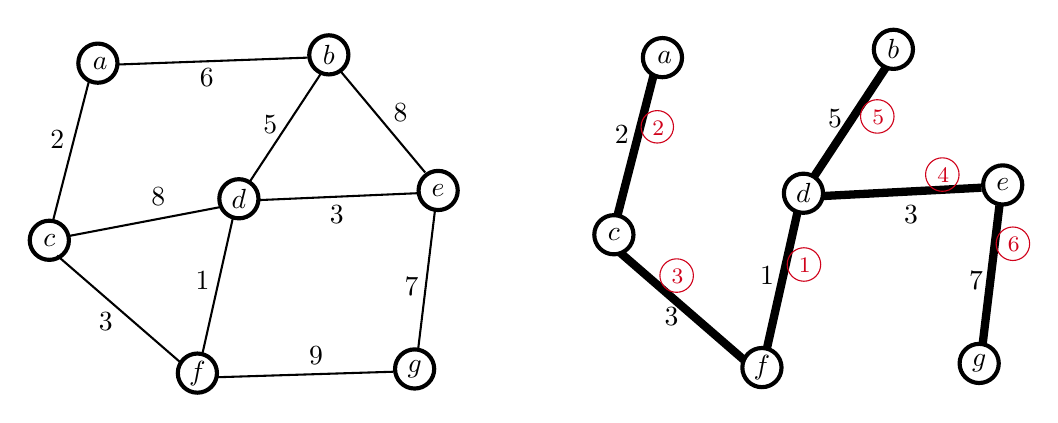
\begin{tikzpicture}[x=0.5pt,y=0.5pt,yscale=-1,xscale=1]
%uncomment if require: \path (0,294); %set diagram left start at 0, and has height of 294

%Straight Lines [id:da6859712806144006] 
\draw [color={rgb, 255:red, 0; green, 0; blue, 0 }  ,draw opacity=1 ][line width=0.75]    (237,42) -- (298,115) ;
%Straight Lines [id:da43828905709564314] 
\draw [color={rgb, 255:red, 0; green, 0; blue, 0 }  ,draw opacity=1 ][line width=0.75]    (147,263) -- (275,259) ;
%Straight Lines [id:da6385368954330931] 
\draw [color={rgb, 255:red, 0; green, 0; blue, 0 }  ,draw opacity=1 ][line width=0.75]    (32,175) -- (122,253) ;
%Straight Lines [id:da061278223687582845] 
\draw [color={rgb, 255:red, 0; green, 0; blue, 0 }  ,draw opacity=1 ][line width=0.75]    (40,161) -- (150,140) ;
%Straight Lines [id:da125058897644165] 
\draw [color={rgb, 255:red, 0; green, 0; blue, 0 }  ,draw opacity=1 ][line width=0.75]    (55,49) -- (29,150) ;
%Straight Lines [id:da7561477389708726] 
\draw [color={rgb, 255:red, 0; green, 0; blue, 0 }  ,draw opacity=1 ][line width=0.75]    (75,37) -- (213,32) ;
%Straight Lines [id:da8045438090716241] 
\draw [color={rgb, 255:red, 0; green, 0; blue, 0 }  ,draw opacity=1 ][line width=0.75]    (223,43) -- (171,122) ;
%Straight Lines [id:da7384444755679203] 
\draw [color={rgb, 255:red, 0; green, 0; blue, 0 }  ,draw opacity=1 ][line width=0.75]    (159,148) -- (137,246) ;
%Straight Lines [id:da7781378597799559] 
\draw [color={rgb, 255:red, 0; green, 0; blue, 0 }  ,draw opacity=1 ][line width=0.75]    (305,143) -- (293,242) ;
%Straight Lines [id:da6283012441188964] 
\draw [color={rgb, 255:red, 0; green, 0; blue, 0 }  ,draw opacity=1 ][line width=0.75]    (292,130) -- (177,135) ;
%Straight Lines [id:da8730022909148112] 
\draw [color={rgb, 255:red, 0; green, 0; blue, 0 }  ,draw opacity=1 ][line width=3]    (586,132) -- (700,126) ;
%Straight Lines [id:da5161692873874864] 
\draw [color={rgb, 255:red, 0; green, 0; blue, 0 }  ,draw opacity=1 ][line width=3]    (463,45) -- (437,146) ;
%Straight Lines [id:da4352724287531199] 
\draw [color={rgb, 255:red, 0; green, 0; blue, 0 }  ,draw opacity=1 ][line width=3]    (631,39) -- (579,118) ;
%Straight Lines [id:da4878171039675874] 
\draw [color={rgb, 255:red, 0; green, 0; blue, 0 }  ,draw opacity=1 ][line width=3]    (567,144) -- (545,242) ;
%Straight Lines [id:da9647292972064201] 
\draw [color={rgb, 255:red, 0; green, 0; blue, 0 }  ,draw opacity=1 ][line width=3]    (713,139) -- (701,238) ;
%Straight Lines [id:da358430115249718] 
\draw [color={rgb, 255:red, 0; green, 0; blue, 0 }  ,draw opacity=1 ][line width=3]    (439,173) -- (529,251) ;

% Text Node
\draw  [line width=1.5]   (307.38, 128) circle [x radius= 14.15, y radius= 14.15]   ;
\draw (307.38,128) node   [align=left] {$\displaystyle e$};
% Text Node
\draw  [line width=1.5]   (61.48, 36) circle [x radius= 14.15, y radius= 14.15]   ;
\draw (55.98,36) node [anchor=west] [inner sep=0.75pt]   [align=left] {$\displaystyle a$};
% Text Node
\draw  [line width=1.5]   (228.38, 30) circle [x radius= 14.15, y radius= 14.15]   ;
\draw (228.38,30) node   [align=left] {$\displaystyle b$};
% Text Node
\draw  [line width=1.5]   (26.38, 164) circle [x radius= 14.15, y radius= 14.15]   ;
\draw (26.38,164) node   [align=left] {$\displaystyle c$};
% Text Node
\draw  [line width=1.5]   (163.38, 134) circle [x radius= 14.15, y radius= 14.15]   ;
\draw (163.38,134) node   [align=left] {$\displaystyle d$};
% Text Node
\draw  [line width=1.5]   (133.38, 260) circle [x radius= 14.15, y radius= 14.15]   ;
\draw (133.38,260) node   [align=left] {$\displaystyle f$};
% Text Node
\draw  [line width=1.5]   (290.38, 257) circle [x radius= 14.15, y radius= 14.15]   ;
\draw (290.38,257) node   [align=left] {$\displaystyle g$};
% Text Node
\draw (25.24,83.06) node [anchor=north west][inner sep=0.75pt]   [align=left] {$\displaystyle 2$};
% Text Node
\draw (133.24,38.06) node [anchor=north west][inner sep=0.75pt]   [align=left] {$\displaystyle 6$};
% Text Node
\draw (227.24,137.06) node [anchor=north west][inner sep=0.75pt]   [align=left] {$\displaystyle 3$};
% Text Node
\draw (179.24,72.06) node [anchor=north west][inner sep=0.75pt]   [align=left] {$\displaystyle 5$};
% Text Node
\draw (98.24,124.06) node [anchor=north west][inner sep=0.75pt]   [align=left] {$\displaystyle 8$};
% Text Node
\draw (60.24,214.06) node [anchor=north west][inner sep=0.75pt]   [align=left] {$\displaystyle 3$};
% Text Node
\draw (130.24,185.06) node [anchor=north west][inner sep=0.75pt]   [align=left] {$\displaystyle 1$};
% Text Node
\draw (273.24,63.06) node [anchor=north west][inner sep=0.75pt]   [align=left] {$\displaystyle 8$};
% Text Node
\draw (212.24,239.06) node [anchor=north west][inner sep=0.75pt]   [align=left] {$\displaystyle 9$};
% Text Node
\draw (281.24,189) node [anchor=north west][inner sep=0.75pt]   [align=left] {$\displaystyle 7$};
% Text Node
\draw  [line width=1.5]   (715.38, 124) circle [x radius= 14.15, y radius= 14.15]   ;
\draw (715.38,124) node   [align=left] {$\displaystyle e$};
% Text Node
\draw  [line width=1.5]   (469.48, 32) circle [x radius= 14.15, y radius= 14.15]   ;
\draw (463.98,32) node [anchor=west] [inner sep=0.75pt]   [align=left] {$\displaystyle a$};
% Text Node
\draw  [line width=1.5]   (636.38, 26) circle [x radius= 14.15, y radius= 14.15]   ;
\draw (636.38,26) node   [align=left] {$\displaystyle b$};
% Text Node
\draw  [line width=1.5]   (434.38, 160) circle [x radius= 14.15, y radius= 14.15]   ;
\draw (434.38,160) node   [align=left] {$\displaystyle c$};
% Text Node
\draw  [line width=1.5]   (571.38, 130) circle [x radius= 14.15, y radius= 14.15]   ;
\draw (571.38,130) node   [align=left] {$\displaystyle d$};
% Text Node
\draw  [line width=1.5]   (541.38, 256) circle [x radius= 14.15, y radius= 14.15]   ;
\draw (541.38,256) node   [align=left] {$\displaystyle f$};
% Text Node
\draw  [line width=1.5]   (698.38, 253) circle [x radius= 14.15, y radius= 14.15]   ;
\draw (698.38,253) node   [align=left] {$\displaystyle g$};
% Text Node
\draw (433.24,79.06) node [anchor=north west][inner sep=0.75pt]   [align=left] {$\displaystyle 2$};
% Text Node
\draw (642.24,137.06) node [anchor=north west][inner sep=0.75pt]   [align=left] {$\displaystyle 3$};
% Text Node
\draw (587.24,68.06) node [anchor=north west][inner sep=0.75pt]   [align=left] {$\displaystyle 5$};
% Text Node
\draw (538.24,181.06) node [anchor=north west][inner sep=0.75pt]   [align=left] {$\displaystyle 1$};
% Text Node
\draw (689.24,185) node [anchor=north west][inner sep=0.75pt]   [align=left] {$\displaystyle 7$};
% Text Node
\draw  [color={rgb, 255:red, 208; green, 2; blue, 27 }  ,draw opacity=1 ]  (571.74, 181.5) circle [x radius= 12.1, y radius= 12.1]   ;
\draw (566.24,175) node [anchor=north west][inner sep=0.75pt]  [font=\footnotesize,color={rgb, 255:red, 208; green, 2; blue, 27 }  ,opacity=1 ] [align=left] {$\displaystyle 1$};
% Text Node
\draw  [color={rgb, 255:red, 208; green, 2; blue, 27 }  ,draw opacity=1 ]  (465.74, 82) circle [x radius= 11.72, y radius= 11.72]   ;
\draw (460.24,76) node [anchor=north west][inner sep=0.75pt]  [font=\footnotesize,color={rgb, 255:red, 208; green, 2; blue, 27 }  ,opacity=1 ] [align=left] {2};
% Text Node
\draw  [color={rgb, 255:red, 208; green, 2; blue, 27 }  ,draw opacity=1 ]  (624.74, 74.5) circle [x radius= 12.1, y radius= 12.1]   ;
\draw (619.24,68) node [anchor=north west][inner sep=0.75pt]  [font=\footnotesize,color={rgb, 255:red, 208; green, 2; blue, 27 }  ,opacity=1 ] [align=left] {$\displaystyle 5$};
% Text Node
\draw (469.24,211.06) node [anchor=north west][inner sep=0.75pt]   [align=left] {$\displaystyle 3$};
% Text Node
\draw  [color={rgb, 255:red, 208; green, 2; blue, 27 }  ,draw opacity=1 ]  (479.74, 189.5) circle [x radius= 12.1, y radius= 12.1]   ;
\draw (474.24,183) node [anchor=north west][inner sep=0.75pt]  [font=\footnotesize,color={rgb, 255:red, 208; green, 2; blue, 27 }  ,opacity=1 ] [align=left] {$\displaystyle 3$};
% Text Node
\draw  [color={rgb, 255:red, 208; green, 2; blue, 27 }  ,draw opacity=1 ]  (671.74, 116.5) circle [x radius= 12.1, y radius= 12.1]   ;
\draw (666.24,110) node [anchor=north west][inner sep=0.75pt]  [font=\footnotesize,color={rgb, 255:red, 208; green, 2; blue, 27 }  ,opacity=1 ] [align=left] {$\displaystyle 4$};
% Text Node
\draw  [color={rgb, 255:red, 208; green, 2; blue, 27 }  ,draw opacity=1 ]  (722.74, 166.5) circle [x radius= 12.1, y radius= 12.1]   ;
\draw (717.24,160) node [anchor=north west][inner sep=0.75pt]  [font=\footnotesize,color={rgb, 255:red, 208; green, 2; blue, 27 }  ,opacity=1 ] [align=left] {$\displaystyle 6$};


\end{tikzpicture}

}
\caption{Running Kruskal's algorithm. The cycled numbers give the order edges are picked.}
\label{fig:mst1}
\end{figure}

\subsection*{Prim's Algorithm}

Prim's algorithm combines the greedy strategy~(i.e., pick the smallest edge whenever possible)
and the 2nd way to construct a spanning tree~(i.e., pick $(|V|-1)$ edges that connects all vertices).
To connect all vertices, we can start from an \emph{arbitrary} vertex and iteratively
make it connected to all other vertices. As we need to use $(|V| - 1)$ edges to connect
to all other $(|V|-1)$ vertices, therefore every edge we pick needs to be connected to a
\emph{new} vertex.
Prim's algorithm can be summarized as: \emph{iteratively pick $(|V|-1)$ edges,
and in each iteration, pick the smallest edge that connects to a new vertex}.
We again use $E_1$ to store the picked edges.
We also use $S$ to store the vertices that have been connected.
The pseudo-code is given below.  See an example in Figure~\ref{fig:mst2}.

\begin{minipage}{0.8\textwidth}
	\aaA {8}{Algorithm Prim's~(graph $G = (V, E)$)}\xxx
	\aab {init $E_1 = \emptyset$;}\xxx
	\aab {init $S$ with an arbitrarily picked vertex;}\xxx
	\aaB {4}{for $k = 1 \to |V| - 1$}\xxx
	\aac {pick the smallest edge $e = (u,v)$ that connects to a new vertex~(i.e., $u\in S$ and $v\not\in S$);}\xxx
	\aac {$E_1 = E_1\cup\{e\}$;}\xxx
	\aac {$S = S\cup\{v\}$;}\xxx
	\aab {end for;}\xxx
	\aaa {end algorithm;}\xxx
\end{minipage}

\begin{figure}[h]
\centering{

\tikzset{every picture/.style={line width=0.75pt}} %set default line width to 0.75pt        

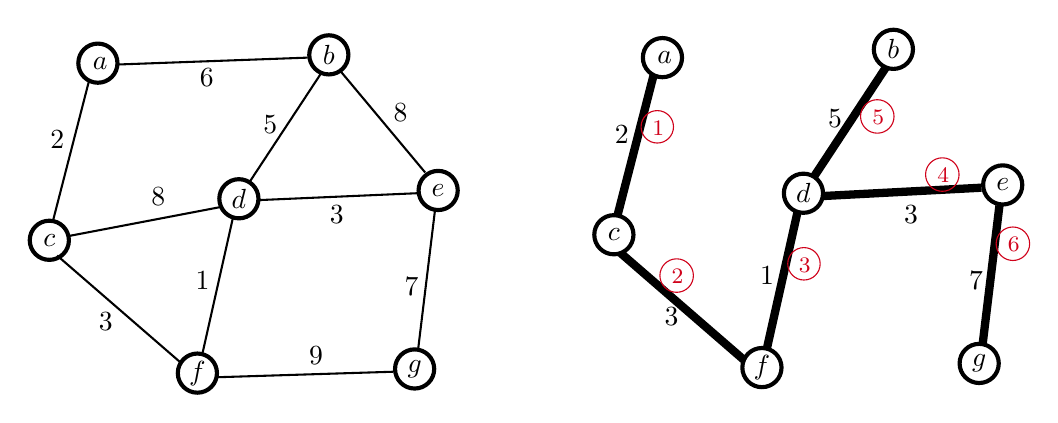
\begin{tikzpicture}[x=0.5pt,y=0.5pt,yscale=-1,xscale=1]
%uncomment if require: \path (0,294); %set diagram left start at 0, and has height of 294

%Straight Lines [id:da6859712806144006] 
\draw [color={rgb, 255:red, 0; green, 0; blue, 0 }  ,draw opacity=1 ][line width=0.75]    (237,42) -- (298,115) ;
%Straight Lines [id:da43828905709564314] 
\draw [color={rgb, 255:red, 0; green, 0; blue, 0 }  ,draw opacity=1 ][line width=0.75]    (147,263) -- (275,259) ;
%Straight Lines [id:da6385368954330931] 
\draw [color={rgb, 255:red, 0; green, 0; blue, 0 }  ,draw opacity=1 ][line width=0.75]    (32,175) -- (122,253) ;
%Straight Lines [id:da061278223687582845] 
\draw [color={rgb, 255:red, 0; green, 0; blue, 0 }  ,draw opacity=1 ][line width=0.75]    (40,161) -- (150,140) ;
%Straight Lines [id:da125058897644165] 
\draw [color={rgb, 255:red, 0; green, 0; blue, 0 }  ,draw opacity=1 ][line width=0.75]    (55,49) -- (29,150) ;
%Straight Lines [id:da7561477389708726] 
\draw [color={rgb, 255:red, 0; green, 0; blue, 0 }  ,draw opacity=1 ][line width=0.75]    (75,37) -- (213,32) ;
%Straight Lines [id:da8045438090716241] 
\draw [color={rgb, 255:red, 0; green, 0; blue, 0 }  ,draw opacity=1 ][line width=0.75]    (223,43) -- (171,122) ;
%Straight Lines [id:da7384444755679203] 
\draw [color={rgb, 255:red, 0; green, 0; blue, 0 }  ,draw opacity=1 ][line width=0.75]    (159,148) -- (137,246) ;
%Straight Lines [id:da7781378597799559] 
\draw [color={rgb, 255:red, 0; green, 0; blue, 0 }  ,draw opacity=1 ][line width=0.75]    (305,143) -- (293,242) ;
%Straight Lines [id:da6283012441188964] 
\draw [color={rgb, 255:red, 0; green, 0; blue, 0 }  ,draw opacity=1 ][line width=0.75]    (292,130) -- (177,135) ;
%Straight Lines [id:da8730022909148112] 
\draw [color={rgb, 255:red, 0; green, 0; blue, 0 }  ,draw opacity=1 ][line width=3]    (586,132) -- (700,126) ;
%Straight Lines [id:da5161692873874864] 
\draw [color={rgb, 255:red, 0; green, 0; blue, 0 }  ,draw opacity=1 ][line width=3]    (463,45) -- (437,146) ;
%Straight Lines [id:da4352724287531199] 
\draw [color={rgb, 255:red, 0; green, 0; blue, 0 }  ,draw opacity=1 ][line width=3]    (631,39) -- (579,118) ;
%Straight Lines [id:da4878171039675874] 
\draw [color={rgb, 255:red, 0; green, 0; blue, 0 }  ,draw opacity=1 ][line width=3]    (567,144) -- (545,242) ;
%Straight Lines [id:da9647292972064201] 
\draw [color={rgb, 255:red, 0; green, 0; blue, 0 }  ,draw opacity=1 ][line width=3]    (713,139) -- (701,238) ;
%Straight Lines [id:da358430115249718] 
\draw [color={rgb, 255:red, 0; green, 0; blue, 0 }  ,draw opacity=1 ][line width=3]    (439,173) -- (529,251) ;

% Text Node
\draw  [line width=1.5]   (307.38, 128) circle [x radius= 14.15, y radius= 14.15]   ;
\draw (307.38,128) node   [align=left] {$\displaystyle e$};
% Text Node
\draw  [line width=1.5]   (61.48, 36) circle [x radius= 14.15, y radius= 14.15]   ;
\draw (55.98,36) node [anchor=west] [inner sep=0.75pt]   [align=left] {$\displaystyle a$};
% Text Node
\draw  [line width=1.5]   (228.38, 30) circle [x radius= 14.15, y radius= 14.15]   ;
\draw (228.38,30) node   [align=left] {$\displaystyle b$};
% Text Node
\draw  [line width=1.5]   (26.38, 164) circle [x radius= 14.15, y radius= 14.15]   ;
\draw (26.38,164) node   [align=left] {$\displaystyle c$};
% Text Node
\draw  [line width=1.5]   (163.38, 134) circle [x radius= 14.15, y radius= 14.15]   ;
\draw (163.38,134) node   [align=left] {$\displaystyle d$};
% Text Node
\draw  [line width=1.5]   (133.38, 260) circle [x radius= 14.15, y radius= 14.15]   ;
\draw (133.38,260) node   [align=left] {$\displaystyle f$};
% Text Node
\draw  [line width=1.5]   (290.38, 257) circle [x radius= 14.15, y radius= 14.15]   ;
\draw (290.38,257) node   [align=left] {$\displaystyle g$};
% Text Node
\draw (25.24,83.06) node [anchor=north west][inner sep=0.75pt]   [align=left] {$\displaystyle 2$};
% Text Node
\draw (133.24,38.06) node [anchor=north west][inner sep=0.75pt]   [align=left] {$\displaystyle 6$};
% Text Node
\draw (227.24,137.06) node [anchor=north west][inner sep=0.75pt]   [align=left] {$\displaystyle 3$};
% Text Node
\draw (179.24,72.06) node [anchor=north west][inner sep=0.75pt]   [align=left] {$\displaystyle 5$};
% Text Node
\draw (98.24,124.06) node [anchor=north west][inner sep=0.75pt]   [align=left] {$\displaystyle 8$};
% Text Node
\draw (60.24,214.06) node [anchor=north west][inner sep=0.75pt]   [align=left] {$\displaystyle 3$};
% Text Node
\draw (130.24,185.06) node [anchor=north west][inner sep=0.75pt]   [align=left] {$\displaystyle 1$};
% Text Node
\draw (273.24,63.06) node [anchor=north west][inner sep=0.75pt]   [align=left] {$\displaystyle 8$};
% Text Node
\draw (212.24,239.06) node [anchor=north west][inner sep=0.75pt]   [align=left] {$\displaystyle 9$};
% Text Node
\draw (281.24,189) node [anchor=north west][inner sep=0.75pt]   [align=left] {$\displaystyle 7$};
% Text Node
\draw  [line width=1.5]   (715.38, 124) circle [x radius= 14.15, y radius= 14.15]   ;
\draw (715.38,124) node   [align=left] {$\displaystyle e$};
% Text Node
\draw  [line width=1.5]   (469.48, 32) circle [x radius= 14.15, y radius= 14.15]   ;
\draw (463.98,32) node [anchor=west] [inner sep=0.75pt]   [align=left] {$\displaystyle a$};
% Text Node
\draw  [line width=1.5]   (636.38, 26) circle [x radius= 14.15, y radius= 14.15]   ;
\draw (636.38,26) node   [align=left] {$\displaystyle b$};
% Text Node
\draw  [line width=1.5]   (434.38, 160) circle [x radius= 14.15, y radius= 14.15]   ;
\draw (434.38,160) node   [align=left] {$\displaystyle c$};
% Text Node
\draw  [line width=1.5]   (571.38, 130) circle [x radius= 14.15, y radius= 14.15]   ;
\draw (571.38,130) node   [align=left] {$\displaystyle d$};
% Text Node
\draw  [line width=1.5]   (541.38, 256) circle [x radius= 14.15, y radius= 14.15]   ;
\draw (541.38,256) node   [align=left] {$\displaystyle f$};
% Text Node
\draw  [line width=1.5]   (698.38, 253) circle [x radius= 14.15, y radius= 14.15]   ;
\draw (698.38,253) node   [align=left] {$\displaystyle g$};
% Text Node
\draw (433.24,79.06) node [anchor=north west][inner sep=0.75pt]   [align=left] {$\displaystyle 2$};
% Text Node
\draw (642.24,137.06) node [anchor=north west][inner sep=0.75pt]   [align=left] {$\displaystyle 3$};
% Text Node
\draw (587.24,68.06) node [anchor=north west][inner sep=0.75pt]   [align=left] {$\displaystyle 5$};
% Text Node
\draw (538.24,181.06) node [anchor=north west][inner sep=0.75pt]   [align=left] {$\displaystyle 1$};
% Text Node
\draw (689.24,185) node [anchor=north west][inner sep=0.75pt]   [align=left] {$\displaystyle 7$};
% Text Node
\draw  [color={rgb, 255:red, 208; green, 2; blue, 27 }  ,draw opacity=1 ]  (571.74, 181) circle [x radius= 11.72, y radius= 11.72]   ;
\draw (566.24,175) node [anchor=north west][inner sep=0.75pt]  [font=\footnotesize,color={rgb, 255:red, 208; green, 2; blue, 27 }  ,opacity=1 ] [align=left] {3};
% Text Node
\draw  [color={rgb, 255:red, 208; green, 2; blue, 27 }  ,draw opacity=1 ]  (465.74, 82) circle [x radius= 11.72, y radius= 11.72]   ;
\draw (460.24,76) node [anchor=north west][inner sep=0.75pt]  [font=\footnotesize,color={rgb, 255:red, 208; green, 2; blue, 27 }  ,opacity=1 ] [align=left] {1};
% Text Node
\draw  [color={rgb, 255:red, 208; green, 2; blue, 27 }  ,draw opacity=1 ]  (624.74, 74.5) circle [x radius= 12.1, y radius= 12.1]   ;
\draw (619.24,68) node [anchor=north west][inner sep=0.75pt]  [font=\footnotesize,color={rgb, 255:red, 208; green, 2; blue, 27 }  ,opacity=1 ] [align=left] {$\displaystyle 5$};
% Text Node
\draw (469.24,211.06) node [anchor=north west][inner sep=0.75pt]   [align=left] {$\displaystyle 3$};
% Text Node
\draw  [color={rgb, 255:red, 208; green, 2; blue, 27 }  ,draw opacity=1 ]  (479.74, 189.5) circle [x radius= 12.1, y radius= 12.1]   ;
\draw (474.24,183) node [anchor=north west][inner sep=0.75pt]  [font=\footnotesize,color={rgb, 255:red, 208; green, 2; blue, 27 }  ,opacity=1 ] [align=left] {$\displaystyle 2$};
% Text Node
\draw  [color={rgb, 255:red, 208; green, 2; blue, 27 }  ,draw opacity=1 ]  (671.74, 116.5) circle [x radius= 12.1, y radius= 12.1]   ;
\draw (666.24,110) node [anchor=north west][inner sep=0.75pt]  [font=\footnotesize,color={rgb, 255:red, 208; green, 2; blue, 27 }  ,opacity=1 ] [align=left] {$\displaystyle 4$};
% Text Node
\draw  [color={rgb, 255:red, 208; green, 2; blue, 27 }  ,draw opacity=1 ]  (722.74, 166.5) circle [x radius= 12.1, y radius= 12.1]   ;
\draw (717.24,160) node [anchor=north west][inner sep=0.75pt]  [font=\footnotesize,color={rgb, 255:red, 208; green, 2; blue, 27 }  ,opacity=1 ] [align=left] {$\displaystyle 6$};


\end{tikzpicture}

}
\caption{Running Prim's algorithm with $S$ being initialized as $\{a\}$. The cycled numbers give the order edges are picked.}
\label{fig:mst2}
\end{figure}


Again the above algorithm is a framework, as how to select the
smallest edge that connects to a new vertex is not specified. 
Later on we will use \emph{priority queue} to efficiently do that.
We also need to prove the correctness of the Prim's algorithm, i.e., it can always find
an MST; we will do that later on.


